%!TEX root = thesis.tex
\chapter{Einleitung}
\label{cha:einleitung}

Keine Überschrift ohne Text $\dots$

\section{Das Lübecker Holstentor}
\label{sec:holstentor}

\subsection{Zitieren}
\label{sec:cite}

Das Eigenbase-Projekt \cite{Akyildiz2008a} ist sehr cool.

\subsection{Grafik}

%See also Grafiken in commands.tex ab Zeile 341 für subfigures etc. 
\begin{figure}[htbp]
	\begin{center}
		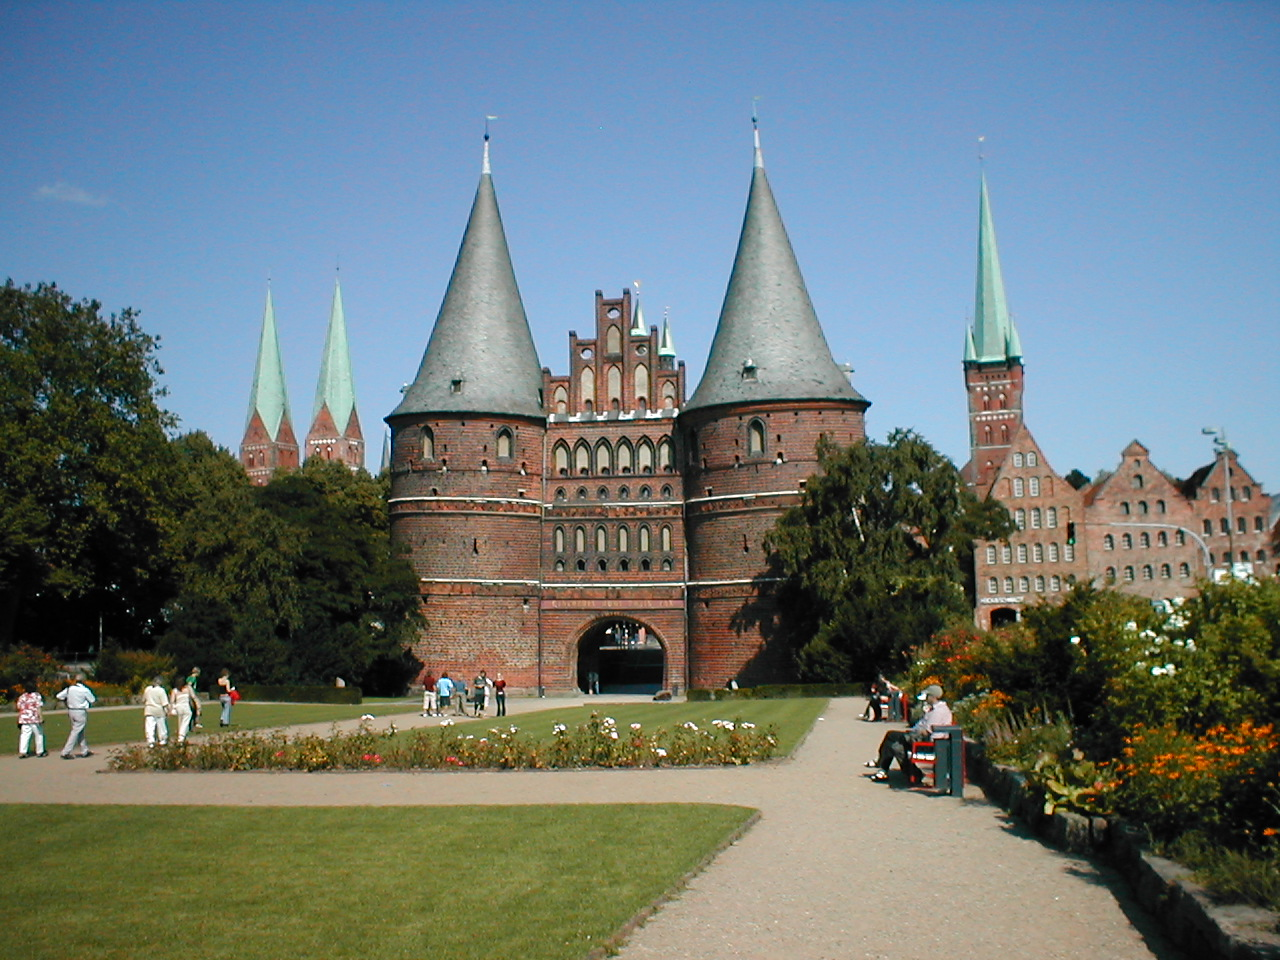
\includegraphics[width=0.75\textwidth]{images/LuebeckHolstentor}
		\caption[Kurzfassung für Abbildungsverzeichnis]{Ausführlicher Titel}
		\label{fig:Holstentor}
		\end{center}
\end{figure}

%Cref ergänzt automatisch Abbildung oder Tabellle etc.
In \Cref{fig:Holstentor} sehen wir das \todo{Eine Randnotiz!} Lübecker Holstentor.

\subsection{Tabelle}

\begin{table}
\centering
\footnotesize
\caption[Kurze Tabellenüberschrift]{Lange Tabellenüberschrift}
\label{tab:eins}
\begin{tabular}{p{1.4cm} p{2.0cm} p{2.0cm}}\toprule
			& A 			& B 		\\[0.1cm]\midrule
	1		& w				& s 		\\[0.2cm]
	2 		& e				& f			\\[0.2cm]
	3		& r				& s			\\[0.2cm]
	4 		& t				& n 		\\\bottomrule
\end{tabular}
\end{table}

In \Cref{tab:eins} sehen wir...

\subsection{Gleichung}

\begin{equation}\label{eq:test}
  a=b
\end{equation}

In \Cref{eq:test} sehen wir...

\subsection{Code-Listing}

\lstinputlisting[label={lst:hello}, caption={This is a code.}]{helloworld.cpp}


In \Cref{lst:hello} wird...

\subsection{Zitat}

Ein Zitat aus der Wikipedia:

\begin{quote}
	\begin{myquote}
		Die Universität zu Lübeck ist eine Hochschule in der Hansestadt Lübeck (Deutschland), die 1964 zunächst als zweite Medizinische Fakultät der Universität Kiel eingerichtet wurde. Studienangebot und Forschungstätigkeit der Universität zu Lübeck haben ihren Ausgangspunkt in der Medizin.
		\label{quote:uni}
	\end{myquote}
\end{quote}

\todo[inline,color=green!40,caption={Kurzversion des Todos}]{Ein Inline-Todo}

%
% Hinweis: CRef funktioniert nicht für Zitate! Bitte \quoteref{...} verwenden
%
In \quoteref{uni}...

\todo[inline]{Mit Besitzer und Datum}

\newpage

Etwas mehr Inhalt auf einer weiteren Seite

\newpage

Etwas mehr Inhalt auf noch einer tollen Seite